\section{Diode Rectifier Circuits}

\subsection{Experiment Design}
    \subsubsection{Background}
        In the previous chapter, we constructed a half wave rectifier. However, the half wave rectifier has a low efficiency and produces a large ripple voltage. In this chapter, we will construct a full wave rectifier to overcome these disadvantages. The full wave rectifier can be constructed in vairious way, in this experiment, we will construct two types of full wave rectifier: the full wave rectifier with center-tapped transformer and the full wave bridge rectifier.

    \subsubsection{Propose}
    \begin{itemize}
        \item To verify a full-wave rectifier with center-tapped transformer
        \item To verify a full-wave bridge rectifier
    \end{itemize}

\subsection{Experiment Design}
    \subsubsection{Materials}
        In this experiment, we will use the following components:
        \begin{itemize}
            \item 1N4148 Diode
            \item Resistors
            \item Transformers
            \item Breadboard
            \item DC power supply
            \item Digital Multi-Meter
            \item Function Generator
            \item Oscilloscope
        \end{itemize}

    \subsubsection{Circuit Diagram}
        The following circuit diagrams 
        \begin{figure}[H]
            \centering
            \begin{subfigure}{0.6\textwidth}
                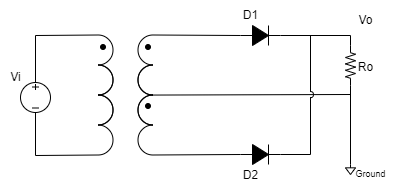
\includegraphics[width=1\linewidth]{Experiment_03/Circuits/Lab3a.png}
                \caption{Center Tapped Full-wave diode rectifier}
                \label{cir:3a}
            \end{subfigure}

            \begin{subfigure}{0.6\textwidth}
                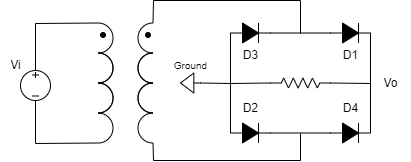
\includegraphics[width=1\linewidth]{Experiment_03/Circuits/Lab3b.png}
                \caption{Bridge Full-wave bridge diode rectifier}
                \label{cir:3b}
            \end{subfigure}
            \caption{Circuit of Diode Rectifier}
        \end{figure}

    \subsubsection{Theoretical Analysis}
        \begin{enumerate}[a]
            \item \textbf{Center Tapped Diode Rectifier}\par
                Center-Tapped Full-wave Rectifier uses two diodes. By using a transformer with two terminal, It split the AC output into two equal halves. And the two diodes conduct during each half of the AC cycle, producing a full-wave rectified output.
            \item \textbf{Bridge Full-wave Rectifier}\par
                Bridge Full-wave Rectifier uses four diodes. During both halves of the AC input cycle, two of the four diodes conduct, ensuring that current flows in the same direction through the load, providing a full-wave rectified output.
        \end{enumerate}

\subsection{Experiment record}
    \subsubsection{Center Tapped Full-wave Rectifier}
    \begin{enumerate}[I]
        \item \textbf{Data Recorded}\newline
            The recorded data for the center-tapped full wave rectifier circuit is shown in the following picture:
            \begin{figure}[h]
                \centering
                \begin{subfigure}[h]{0.4\textwidth}
                    \centering
                    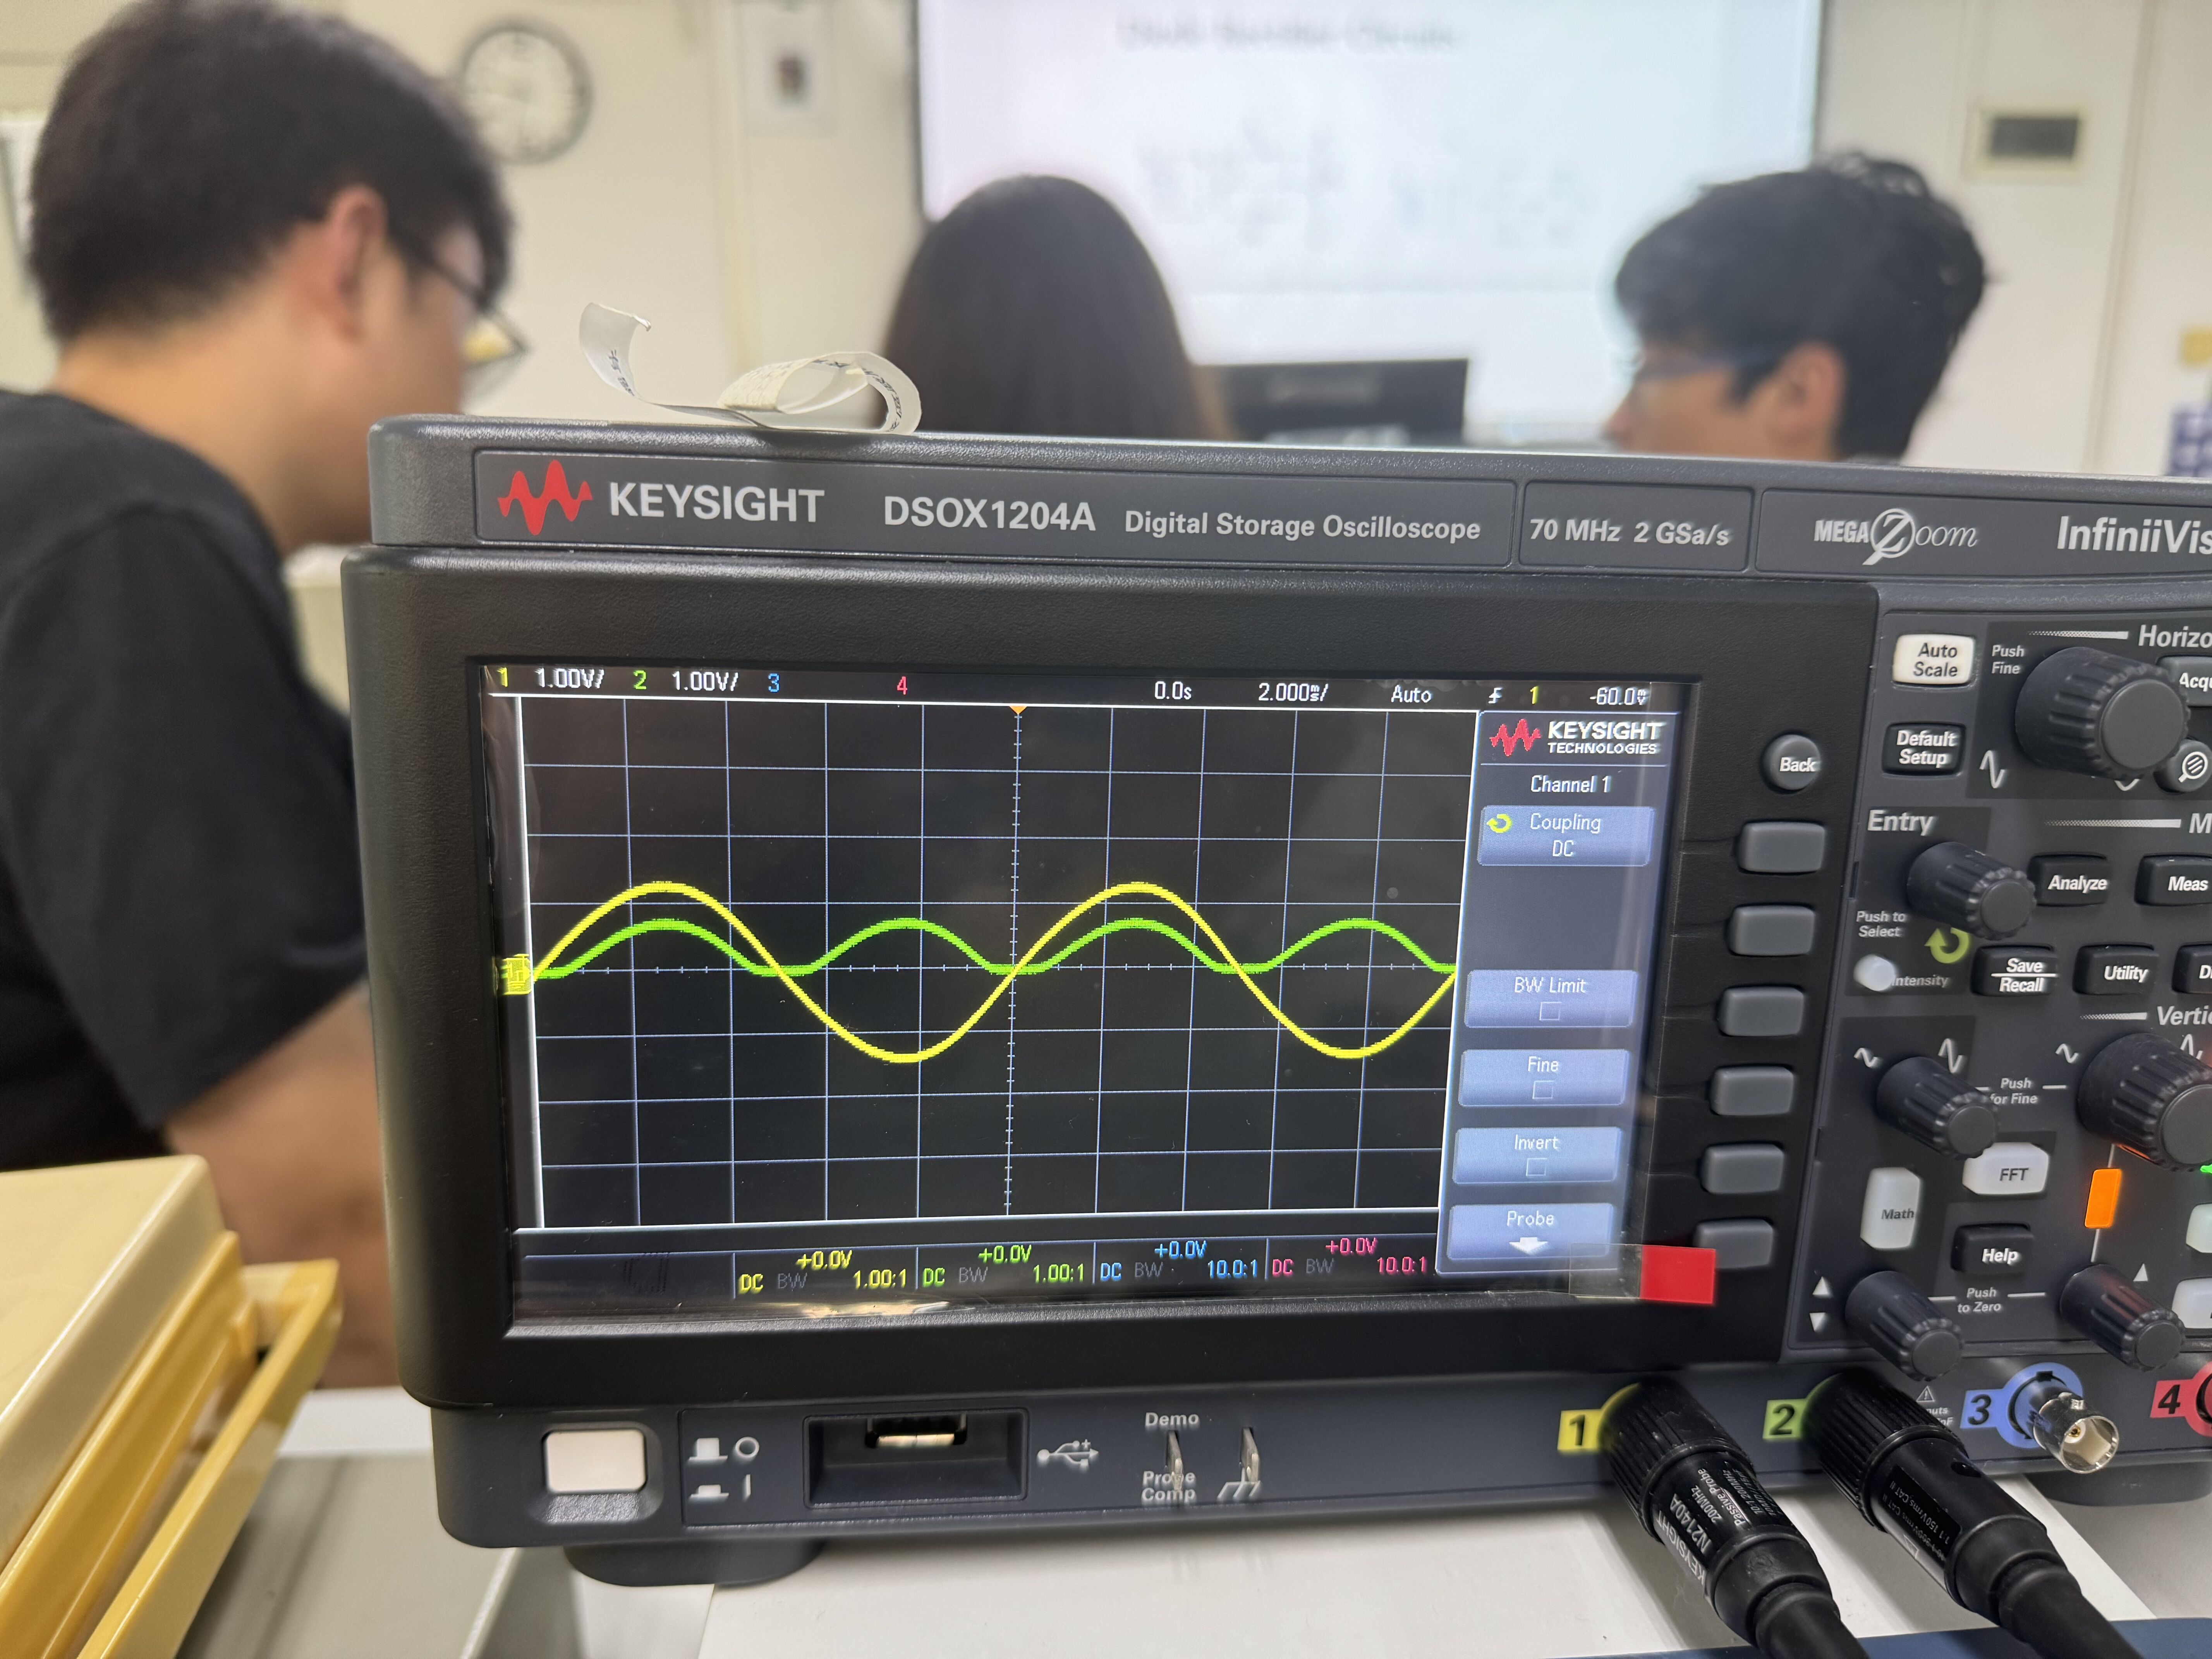
\includegraphics[width=1\textwidth]{Experiment_03/Images/3.4_outPutVoltage.jpg}
                    \caption{Output Voltage}
                    \label{wave:3.4OV}
                \end{subfigure}
                \begin{subfigure}[h]{0.4\textwidth}
                    \centering
                    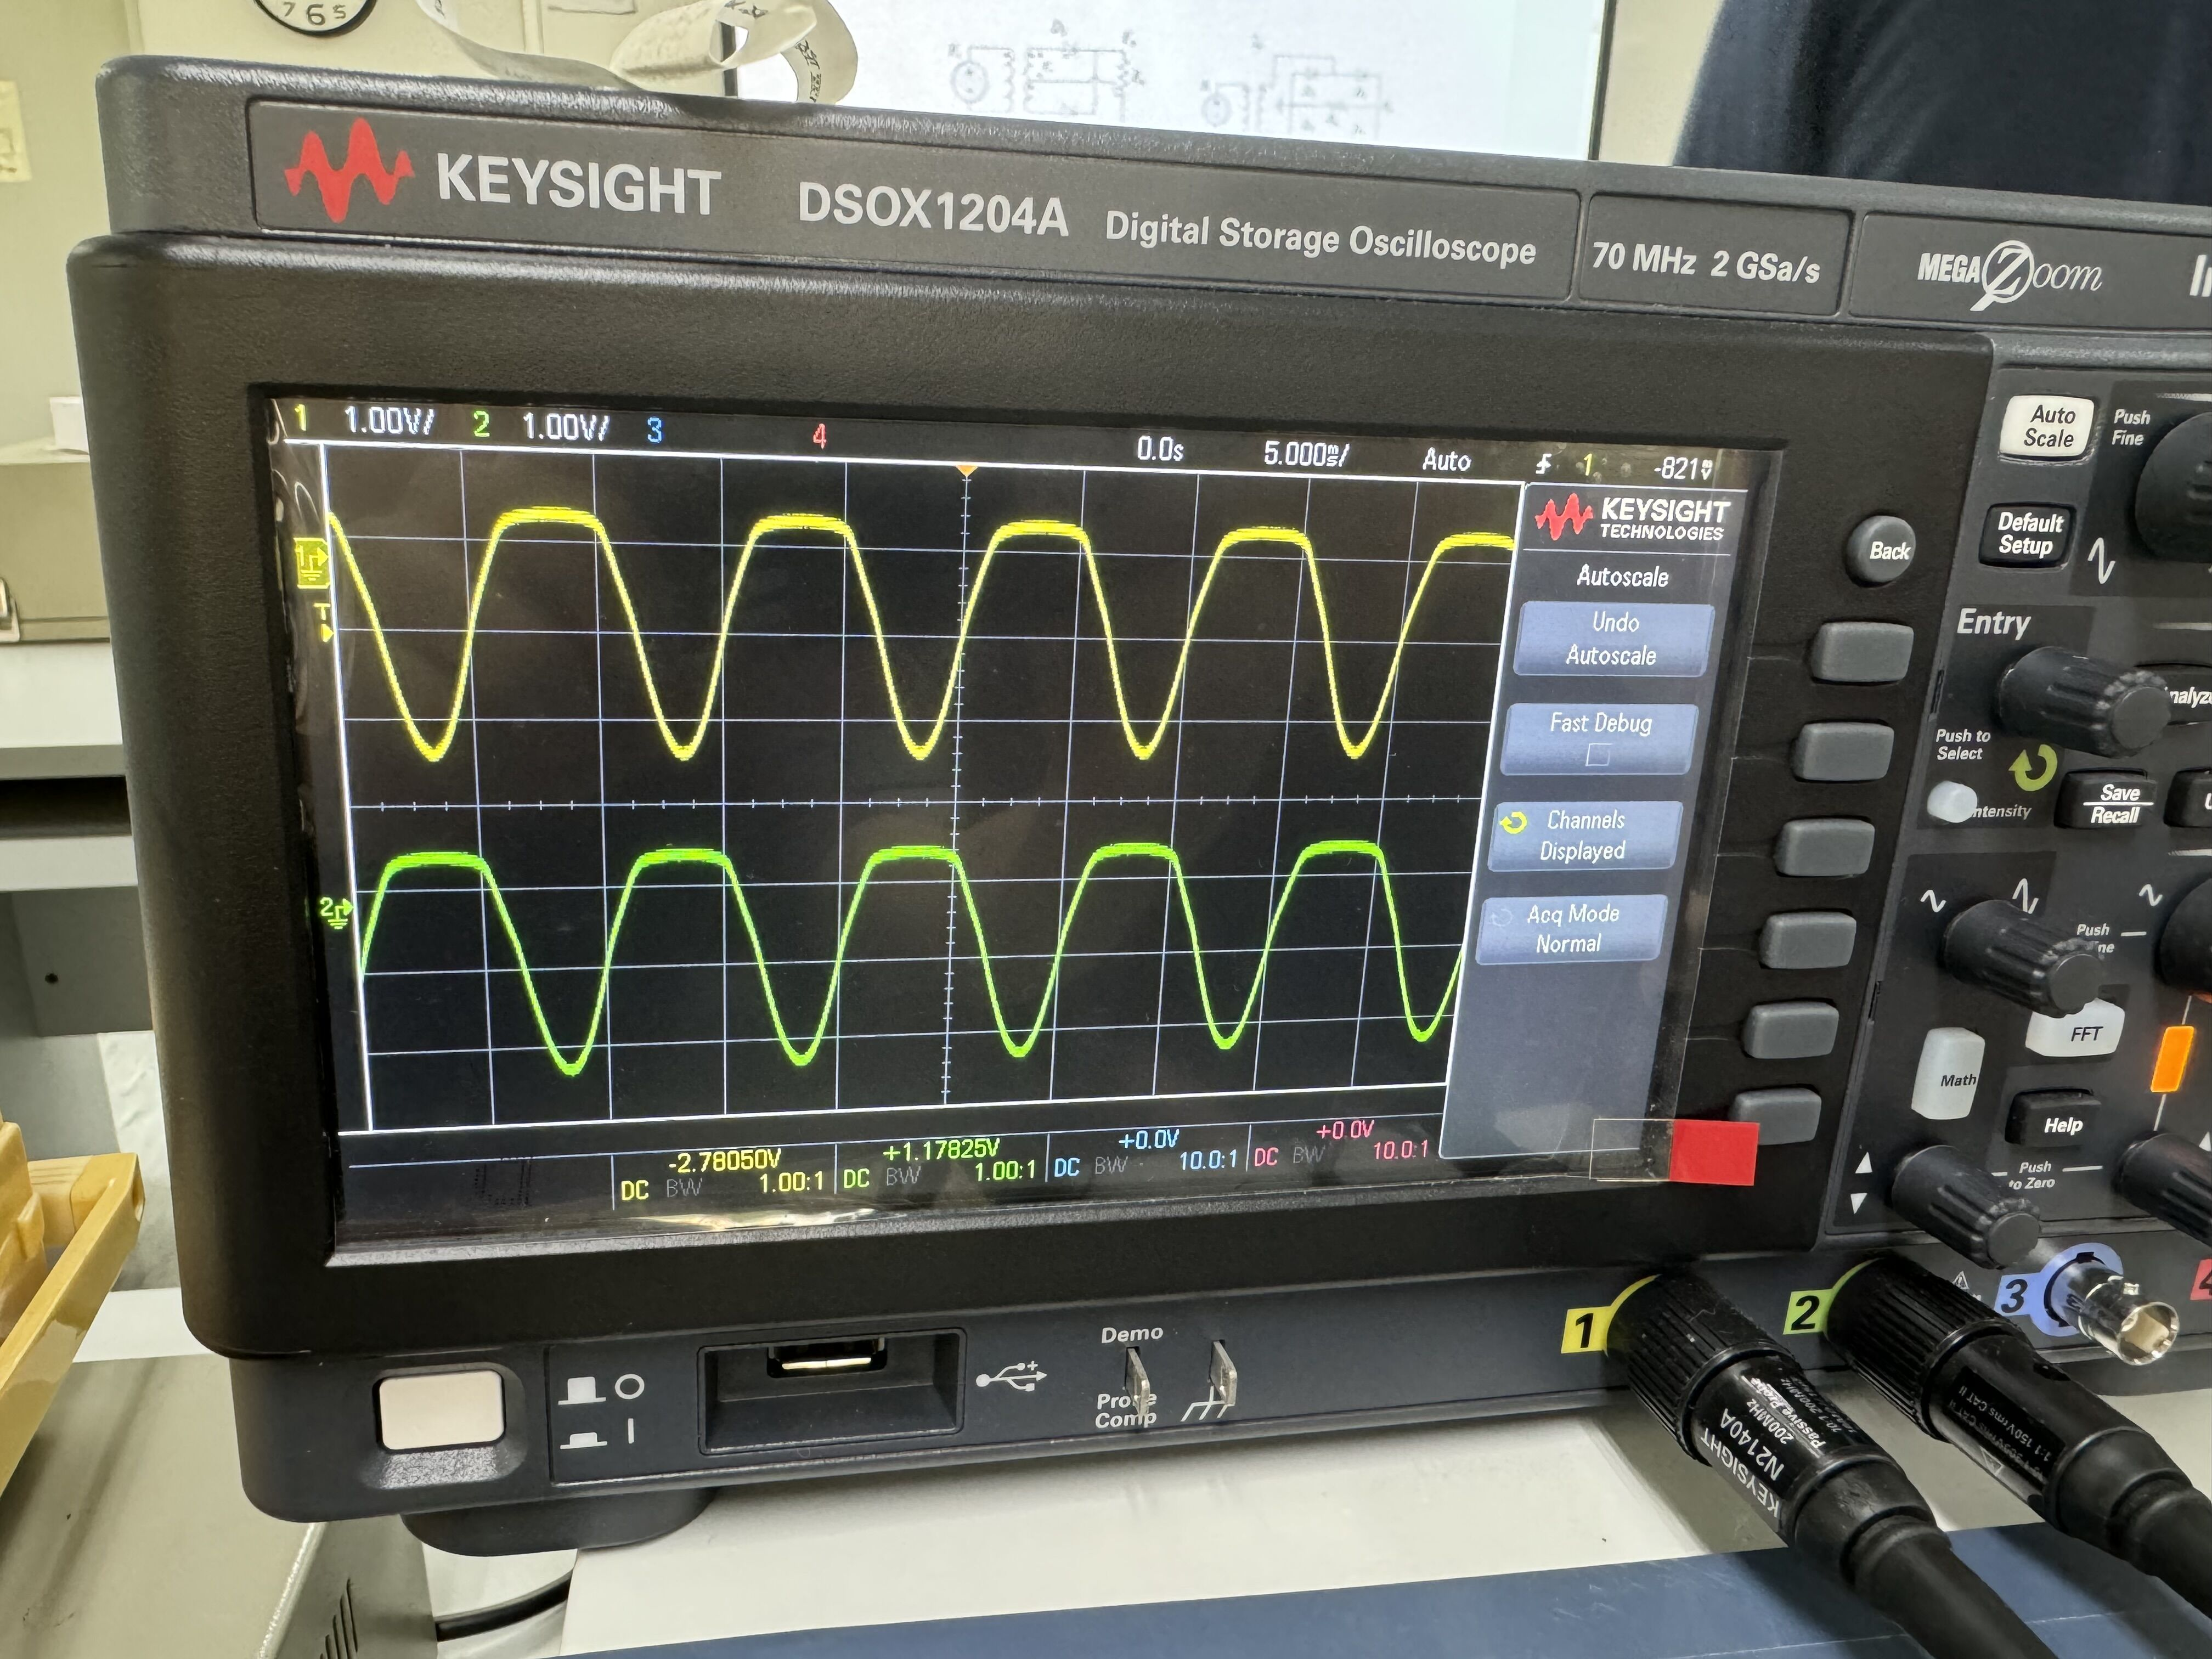
\includegraphics[width=1\textwidth]{Experiment_03/Images/3.4_diodeVoltage.jpg}
                    \caption{Diode Voltage}
                    \label{wave:3.4DV}
                \end{subfigure}
            \end{figure}
        \item \textbf{Data Analysis}\newline
            From Fig.\ref{wave:3.4OV}, we can see the negetive signal from input is flipped, and the output signal have an amplitude about half of the input signal. This is because the Center-Tapped transformer split the input signal into two protion with half of original energy.\par
            
            And Fig.\ref{wave:3.4DV} shows two diodes are working alternatively.
    \end{enumerate}

    \subsubsection{Bridge Full-wave Rectifier}
    \begin{enumerate}[I]
        \item \textbf{Data Recorded}\newline
            The recorded data for the bridge full wave rectifier circuit is shown in the following picture:
            \begin{figure}[h]
                \centering
                \begin{subfigure}[h]{0.4\textwidth}
                    \centering
                    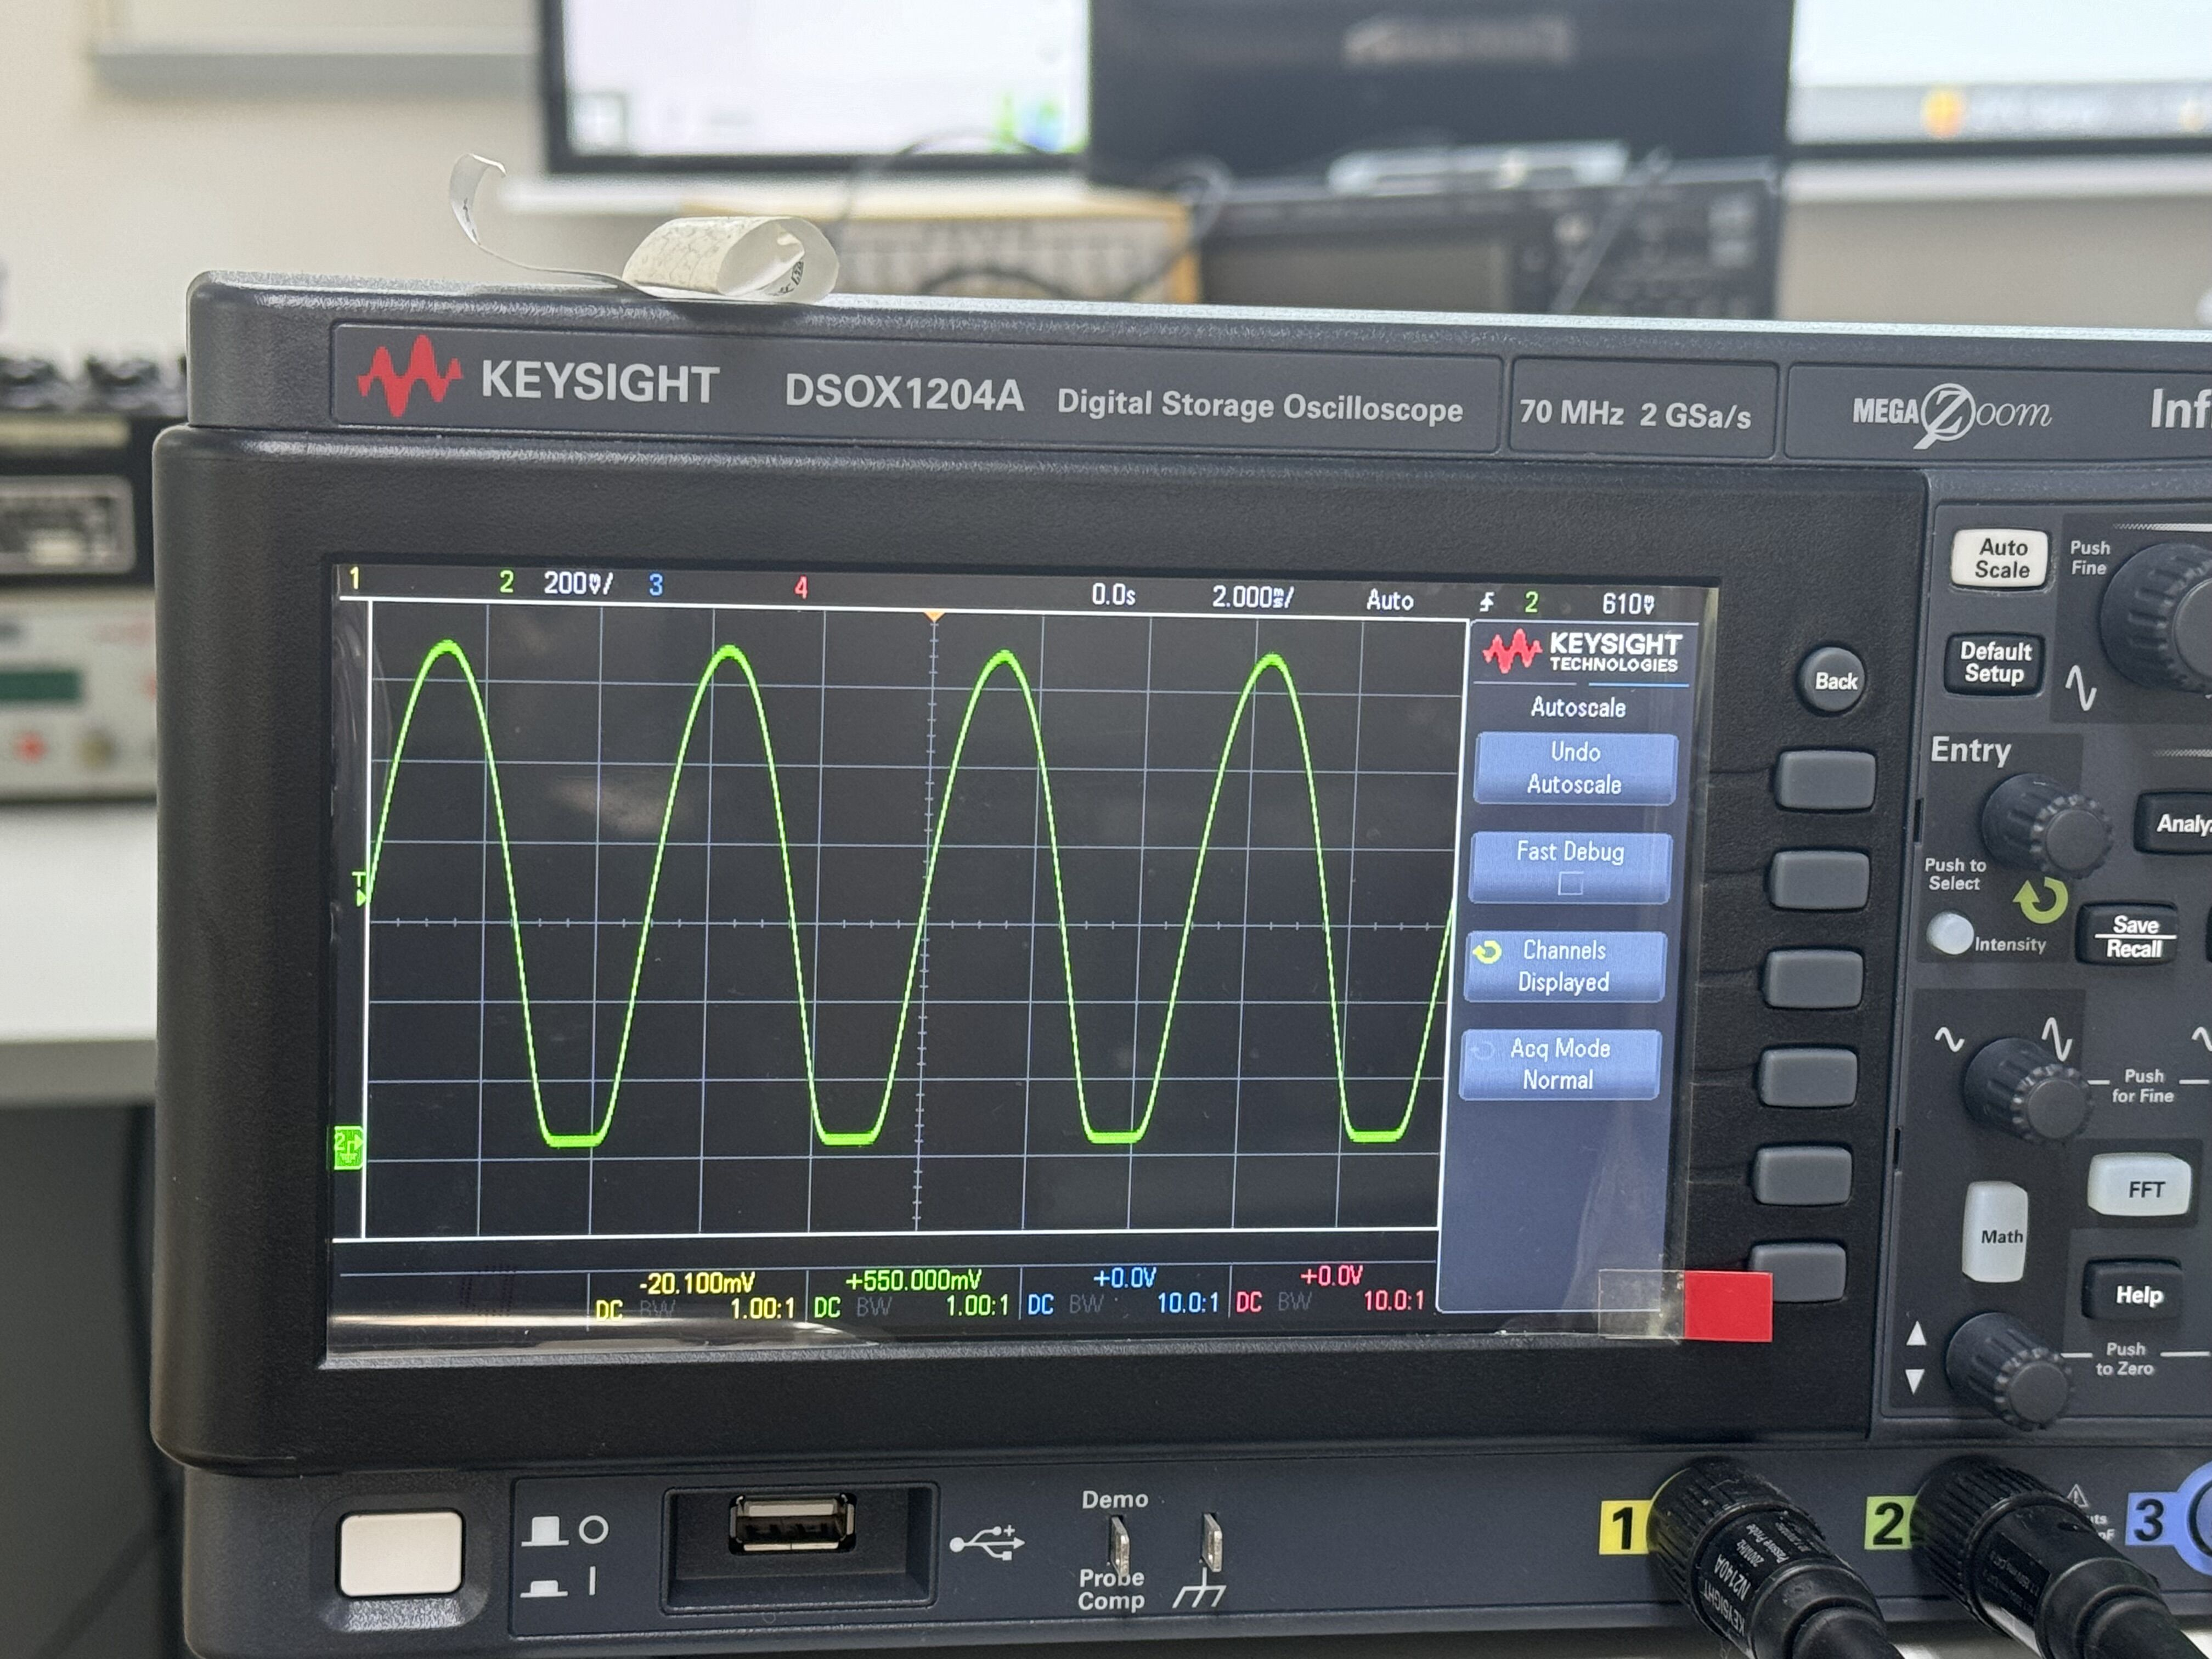
\includegraphics[width=1\textwidth]{Experiment_03/Images/3.5_outPutVoltage.jpg}
                    \caption{Output Voltage}
                    \label{wave:3.5OV}
                \end{subfigure}
                \begin{subfigure}[h]{0.4\textwidth}
                    \centering
                    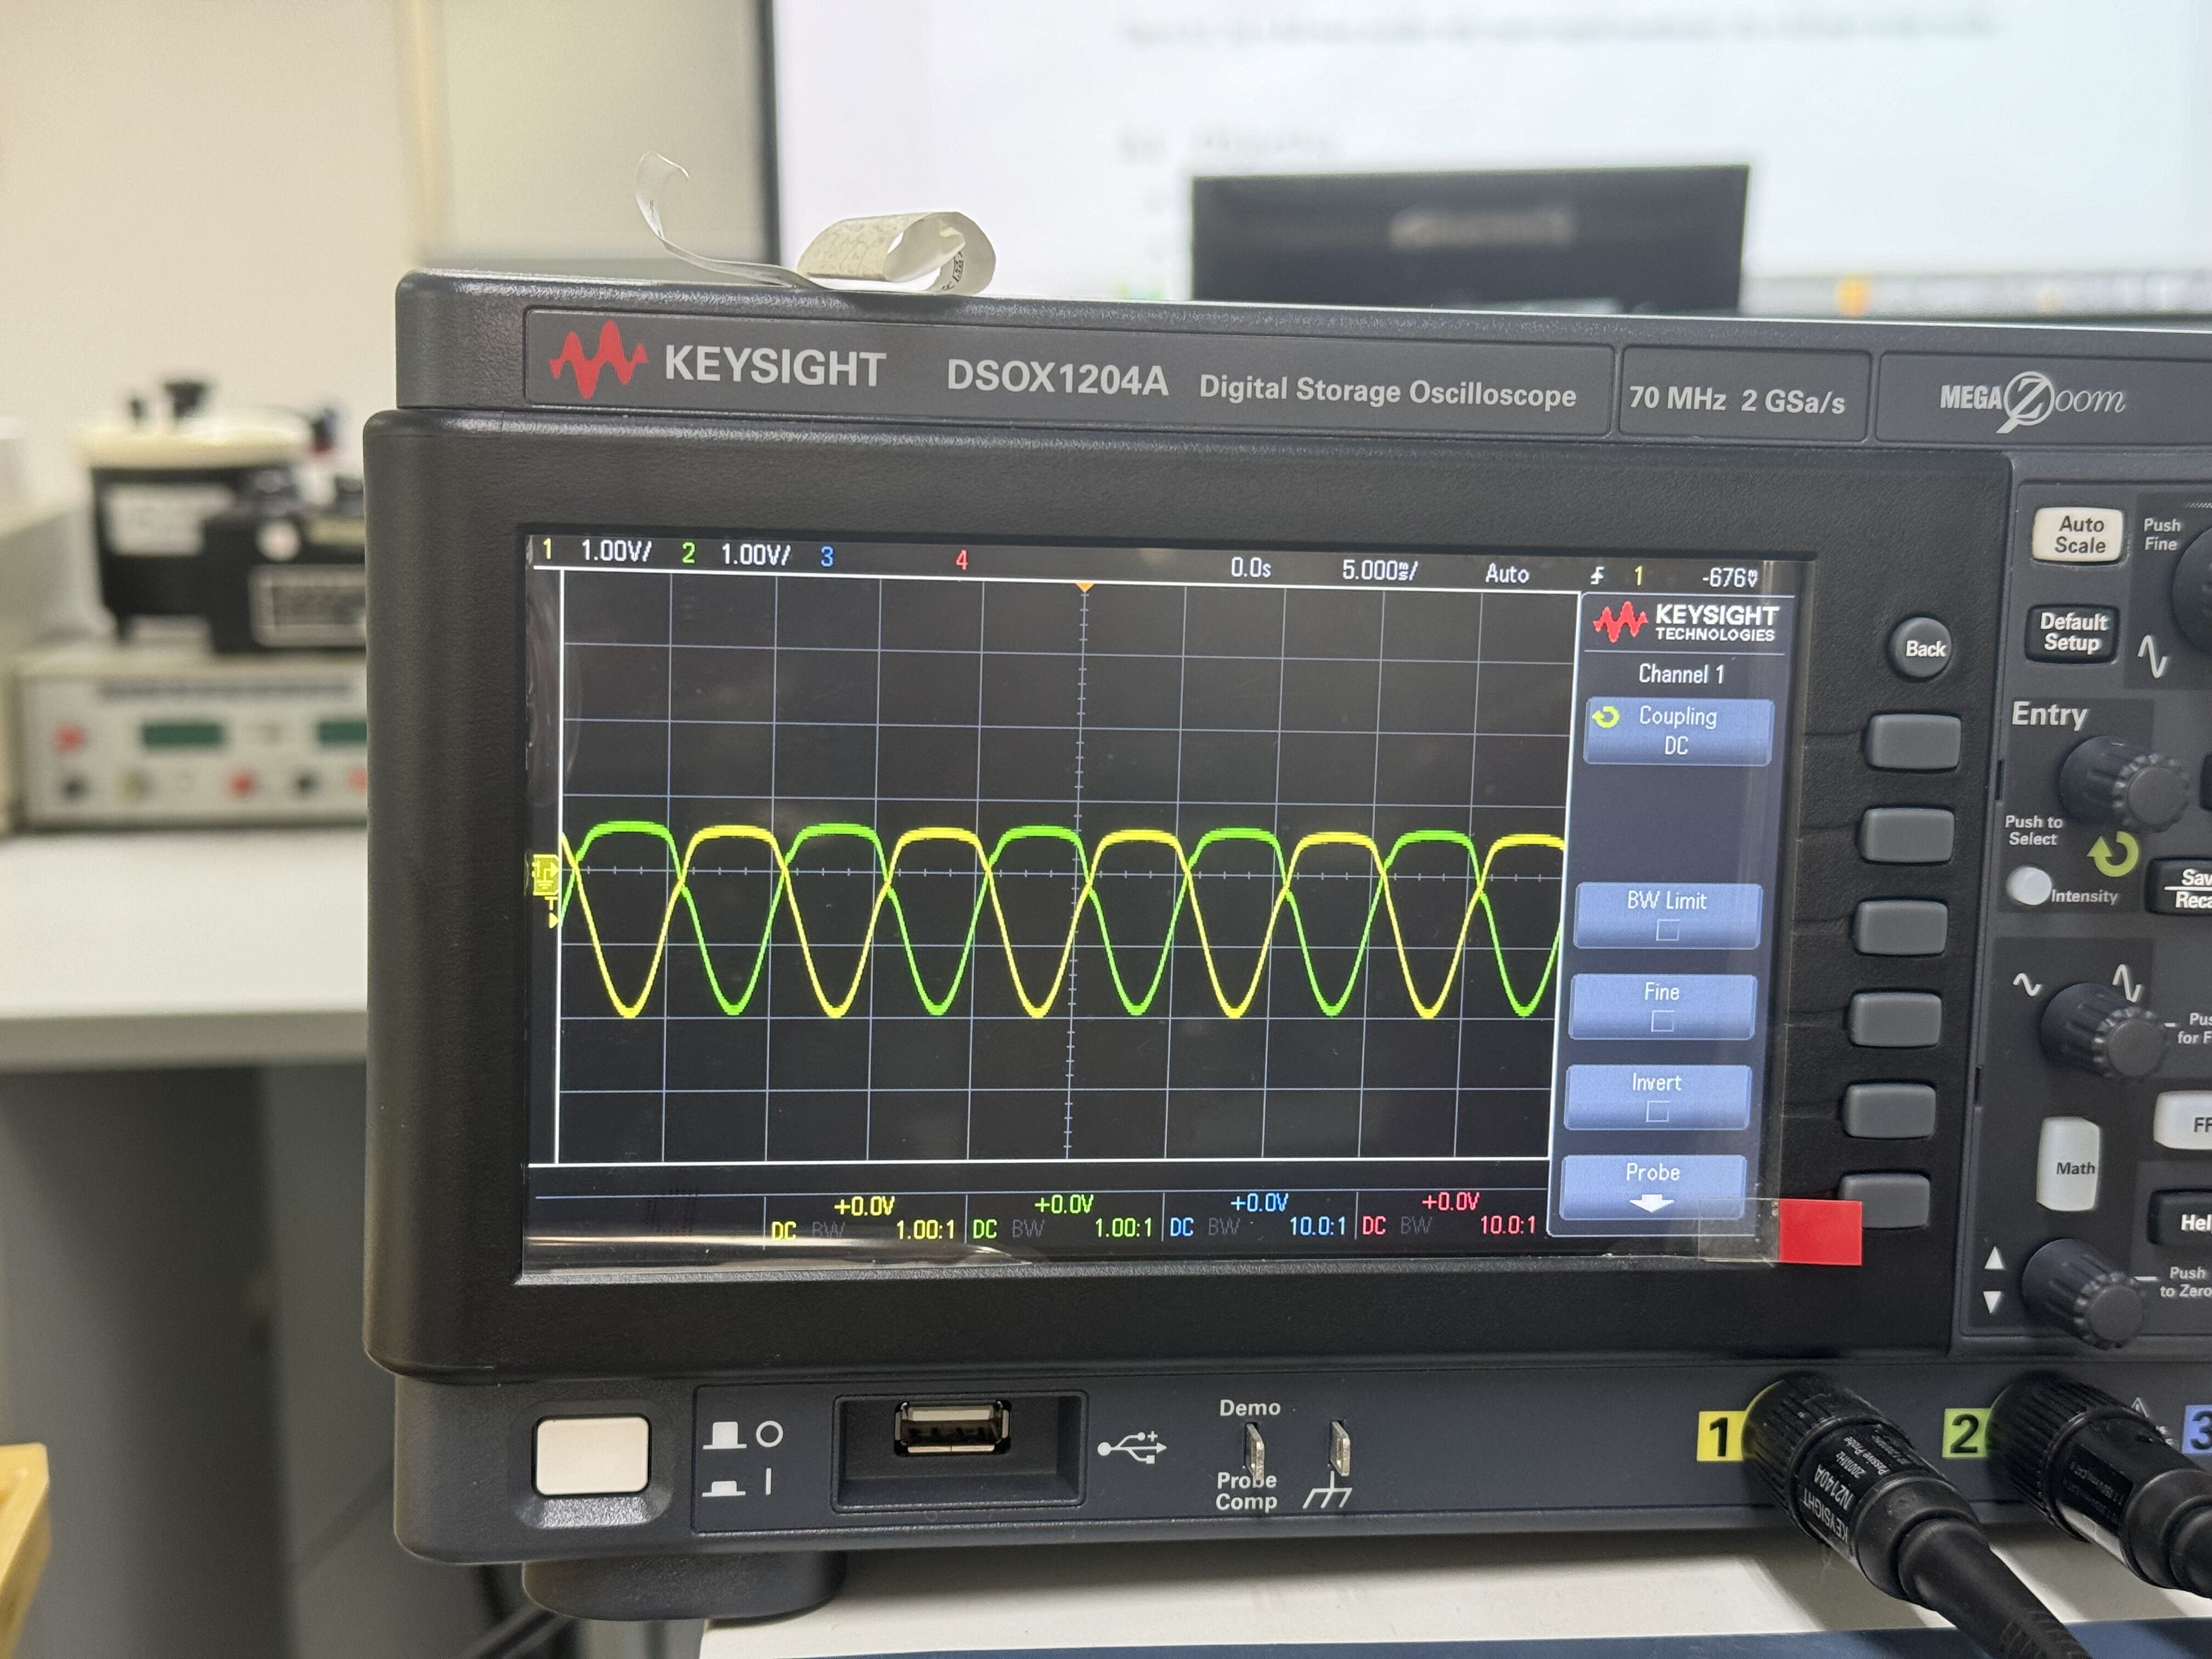
\includegraphics[width=1\textwidth]{Experiment_03/Images/3.5_diodeVoltage.jpg}
                    \caption{Diode Voltage}
                    \label{wave:3.5DV}
                \end{subfigure}
            \end{figure}
        \item \textbf{Data Analysis}\newline
            From Fig.\ref{wave:3.5OV}, we can see the output signal have same amplitude as the original signal. In addition,the output have a smaller ripple voltage than the Center-Tapped Full-wave Rectifier. This is because the Bridge Full-wave Rectifier use four diodes to conduct the current, which provide a more stable output signal.\par
            
            And Fig.\ref{wave:3.5DV} shows the two paires of diodes are working alternatively.
    \end{enumerate}
    
\subsection{Experiment Conclusion}
    \subsubsection{Discussion}
        In this experiment, we notice the Center-Tapped Full-wave Rectifier and Bridge Full-wave Rectifier have different advantage. The Center-Tapped Full-wave Rectifier is chaper and easier to construct, but it has a lower efficiency and produce a larger ripple voltage. On the other hand, the Bridge Full-wave Rectifier is more expensive and complex, but it has a higher efficiency and produce a smaller ripple voltage.
    \subsubsection{Conclusion}